\documentclass{article}\usepackage[]{graphicx}\usepackage[]{xcolor}
% maxwidth is the original width if it is less than linewidth
% otherwise use linewidth (to make sure the graphics do not exceed the margin)
\makeatletter
\def\maxwidth{ %
  \ifdim\Gin@nat@width>\linewidth
    \linewidth
  \else
    \Gin@nat@width
  \fi
}
\makeatother

\definecolor{fgcolor}{rgb}{0.345, 0.345, 0.345}
\newcommand{\hlnum}[1]{\textcolor[rgb]{0.686,0.059,0.569}{#1}}%
\newcommand{\hlsng}[1]{\textcolor[rgb]{0.192,0.494,0.8}{#1}}%
\newcommand{\hlcom}[1]{\textcolor[rgb]{0.678,0.584,0.686}{\textit{#1}}}%
\newcommand{\hlopt}[1]{\textcolor[rgb]{0,0,0}{#1}}%
\newcommand{\hldef}[1]{\textcolor[rgb]{0.345,0.345,0.345}{#1}}%
\newcommand{\hlkwa}[1]{\textcolor[rgb]{0.161,0.373,0.58}{\textbf{#1}}}%
\newcommand{\hlkwb}[1]{\textcolor[rgb]{0.69,0.353,0.396}{#1}}%
\newcommand{\hlkwc}[1]{\textcolor[rgb]{0.333,0.667,0.333}{#1}}%
\newcommand{\hlkwd}[1]{\textcolor[rgb]{0.737,0.353,0.396}{\textbf{#1}}}%
\let\hlipl\hlkwb

\usepackage{framed}
\makeatletter
\newenvironment{kframe}{%
 \def\at@end@of@kframe{}%
 \ifinner\ifhmode%
  \def\at@end@of@kframe{\end{minipage}}%
  \begin{minipage}{\columnwidth}%
 \fi\fi%
 \def\FrameCommand##1{\hskip\@totalleftmargin \hskip-\fboxsep
 \colorbox{shadecolor}{##1}\hskip-\fboxsep
     % There is no \\@totalrightmargin, so:
     \hskip-\linewidth \hskip-\@totalleftmargin \hskip\columnwidth}%
 \MakeFramed {\advance\hsize-\width
   \@totalleftmargin\z@ \linewidth\hsize
   \@setminipage}}%
 {\par\unskip\endMakeFramed%
 \at@end@of@kframe}
\makeatother

\definecolor{shadecolor}{rgb}{.97, .97, .97}
\definecolor{messagecolor}{rgb}{0, 0, 0}
\definecolor{warningcolor}{rgb}{1, 0, 1}
\definecolor{errorcolor}{rgb}{1, 0, 0}
\newenvironment{knitrout}{}{} % an empty environment to be redefined in TeX

\usepackage{alltt}
\usepackage{amsmath} %This allows me to use the align functionality.
                     %If you find yourself trying to replicate
                     %something you found online, ensure you're
                     %loading the necessary packages!
\usepackage{amsfonts}%Math font
\usepackage{graphicx}%For including graphics
\usepackage{hyperref}%For Hyperlinks
\usepackage[shortlabels]{enumitem}% For enumerated lists with labels specified
                                  % We had to run tlmgr_install("enumitem") in R
\hypersetup{colorlinks = true,citecolor=black} %set citations to have black (not green) color
\usepackage{natbib}        %For the bibliography
\setlength{\bibsep}{0pt plus 0.3ex}
\bibliographystyle{apalike}%For the bibliography
\usepackage[margin=0.50in]{geometry}
\usepackage{float}
\usepackage{multicol}

%fix for figures
\usepackage{caption}
\newenvironment{Figure}
  {\par\medskip\noindent\minipage{\linewidth}}
  {\endminipage\par\medskip}
\IfFileExists{upquote.sty}{\usepackage{upquote}}{}
\begin{document}

\vspace{-1in}
\title{Lab XX -- MATH 240 -- Computational Statistics}

\author{
  Sankalp Ojha \\
  Colgate University  \\
  Mathematics  \\
  {\tt sojha@colgate.edu}
}

\date{04/03/2025}

\maketitle

\begin{multicols}{2}
\begin{abstract}
This document provides a basic template for the 2-page labs we will complete each week. Here, briefly summarize what you did and why it might be helpful. Provide all the top-line conclusions, but avoid providing \emph{all} the details. Results should be limited to ``we show X, Y, and Z."
\end{abstract}

\noindent \textbf{Keywords:} What topics does the lab cover concerning class? List 3-4 key terms here, separated by semicolons.

\section{Introduction}
Provide an overarching summary of what you're talking about. In this section, you introduce the idea to the reader, and your goal is to pull them in. What's the mystery you aim to solve?

You want to provide enough background to understand the context of the work. Specifically, what is the question you are addressing? If it applies, describe what information currently exists about this problem, including citations, and explain how the question you're answering complements this work.

\section{Density Functions and Parameters}
The Beta distribution is a continuous distribution. A continuous distribution is one which has probability density function (PDF) and a cumulative density function (CDF) to represent its probability. The Beta distribution has two parameters, $\alpha$ and $\beta$, which dictate on the distribution looks. Both $\alpha$ and $\beta$ are positive numbers and correspond to \texttt{shape1} and \texttt{shape2}, respectively, when write code for the Beta distribution in \texttt{R}.

\[f_X(x|\alpha, \beta) = \frac{\Gamma(\alpha + \beta)}{\Gamma\alpha\Gamma\beta} x^{\alpha-1}(1-x)^{\beta-1}I(x \in [0,1]).\]

\indent In the beta distribution, $I(x \in [0,1]) = 1$ when $x \in [0,1]$ and $0$ whenever $x$ does not hold a number in support on the Beta distribution. The support of a random variable $X$ in the Beta distribution is $[0,1]$.

\section{Properties and Key Statistics}
The Beta distribution is a very versatile and flexible function when it comes to the shapes it can take on based on the various values of the $\alpha$ and $\beta$ parameters. The various forms of the Beta distribution can be shown through statistics such as mean, variance, skewness, and excess kurtosis. Something to note about the \verb|kurt()| function in \texttt{R} is that it computes the excess kurtosis. So, if we are interested in finding kurtosis of a distribution, we can simply add three to the excess kurtosis found through the \verb|kurt()| function. The equations which can be used to calculate the statistics for a Beta distribution are written in terms of $\alpha$ and $\beta$, as seen below:

\begin{align*}
 E(X) = \frac{\alpha}{\alpha + \beta} \tag{The Mean}\\
var(X) = \frac{\alpha\beta}{(\alpha + \beta)^2(\alpha + \beta + 1)} \tag{The Variance} \\
skew(X) = \frac{2(\beta - \alpha)\sqrt{\alpha + \beta + 1}}{(\alpha + \beta + 2)\sqrt{\alpha\beta}} \tag{The Skewness}
\end{align*}
\[kurt(X) = \frac{6[(\alpha - \beta)^2(\alpha + \beta + 1) - \alpha\beta(\alpha + \beta + 2)]}{\alpha\beta(\alpha + \beta + 2)(\alpha + \beta + 3)}\]
\begin{flushright}
(The Excess Kurtosis)
\end{flushright}

Another way to compute these statistics is through their centered and uncentered $k$th moments. We can compute various combinations of centered and uncentered $k$th moments of the Beta distribution to calculate a certain statistic, as seen below:

\begin{align*}
 \mu_X = E(X) \tag{The Mean}\\
 var(X) = \sigma^2_X = E[(X-\mu_X)]^2 \tag{The Variance}\\
 skew(X) = \frac{E[(X - \mu_X)^3]}{E[(X-\mu_X)^2]^{3/2}} \tag{The Skewness}\\
 kurt(X) = \frac{E[(X-\mu_X)^4]}{E[(X-\mu_X)^2]^2} - 3 \tag{The Excess Kurtsosis}
\end{align*}

To generalize these equations to calculate any centered or uncentered $k$th moment of the Beta distribution, we can use the equations

\[E(X^{k}) = \int_{\chi}^{} x^{k}f_x(x) \,dx \]
\begin{center}
and 
\end{center}
\[E((X-\mu_X)^{k}) = \int_{\chi}^{} (x-\mu_X)^{k}f_x(x) \,dx \]

where the first equation corresponds to a centered $k$th moment and the second equation corresponds to a uncentered $k$th moment.

For the purposes of this lab, a function \verb|beta.moment(alpha, beta, k, centered)| was made to calculate the various statistics of the Beta distribution for various values of $\alpha$ and $\beta$.

\subsection{Power of Larger Sample Sizes}
By generating a large random sample from a from a fixed Beta distribution with parameters $\alpha = 2$ and $\beta = 5$, we were able to prove that larger random sample sizes converge closer to the exact distribution. Using the \texttt{cumstats} package \cite{cumstats}, a figure illustrates how the Weak Law Of Large Numbers, which states that as the sample size increases so will the precision increase towards the total population distribution.

\section{Estimators And Checking Precision}
When dealing with data in real world applications, we don't necessarily know what the values of the parameters $\alpha$ and $\beta$ will be for the given data set. This is where we use point estimators to calculate the precise values of $\alpha$ and $\beta$ which will best fit the data set. The two methods to estimate include: Method of Moments (MOM) and Maximum Likelihood Estimation (MLE). The MOM approach equates the first sample $k$th moments to the first population $k$th moments. The goal is to find which values of $\alpha$ and $\beta$ will match the data set moments best with the population moments. The MLE approach utilizes a likelihood function which aims to find the values of $\alpha$ and $\beta$ which will maximize the likelihood of matching the shape given data set. Ås both of these methods are estimates, we would like to know how precise the estimates are, which we can do through caluculating Bias, Prescision, and Mean Squared Error (MSE). Bias caluculates the average difference from the true value, precision calculates the consistency of the estimates, and MSE combines both prior metrics to calculate the error. The equations to calculate each measure are:

\[\text{Bias} = \mathbb{E}(\hat{\theta}) - \theta\]
\[\text{Precision} = \frac{1}{\text{Var}(\hat{\theta})}\]
\[\text{MSE} = \text{Var}(\hat{\theta}) + \left( \mathbb{E}(\hat{\theta}) - \theta \right)^2\]

\noindent where $\boldsymbol{\hat{\theta}}$ is a given vector of estimates and $\boldsymbol{\theta}$ is the true value.

%%%%%%%%%%%%%%%%%%%%%%%%%%%%%%%%%%%%%%%%%%%%%%%%%%%%%%%%%%%%%%%%%%%%%%%%%%%%%%%%
% Bibliography
%%%%%%%%%%%%%%%%%%%%%%%%%%%%%%%%%%%%%%%%%%%%%%%%%%%%%%%%%%%%%%%%%%%%%%%%%%%%%%%%
\vspace{2em}

\noindent\textbf{Bibliography:} Note that when you add citations to your bib.bib file \emph{and}
you cite them in your document, the bibliography section will automatically populate here.

\begin{tiny}
\bibliography{bib7}
\end{tiny}
\end{multicols}

%%%%%%%%%%%%%%%%%%%%%%%%%%%%%%%%%%%%%%%%%%%%%%%%%%%%%%%%%%%%%%%%%%%%%%%%%%%%%%%%
% Appendix
%%%%%%%%%%%%%%%%%%%%%%%%%%%%%%%%%%%%%%%%%%%%%%%%%%%%%%%%%%%%%%%%%%%%%%%%%%%%%%%%
\newpage
\onecolumn
\section{Appendix}

\begin{table}[ht]
\centering
\caption{Population Summary Of 4 Beta Distribution Parameters}
\label{table1}
\begin{tabular}{rrrrrrr}
  \hline
 & Alpha & Beta & Mean & Variance & Skewness & Excess Kurtosis \\ 
  \hline
1 & 2.00 & 5.00 & 0.29 & 0.03 & 0.60 & -0.12 \\ 
  2 & 5.00 & 5.00 & 0.50 & 0.02 & 0.00 & -0.46 \\ 
  3 & 5.00 & 2.00 & 0.71 & 0.03 & -0.60 & -0.12 \\ 
  4 & 0.50 & 0.50 & 0.50 & 0.12 & 0.00 & -1.50 \\ 
   \hline
\end{tabular}
\end{table}

\begin{figure}[ht]
  \begin{center}
  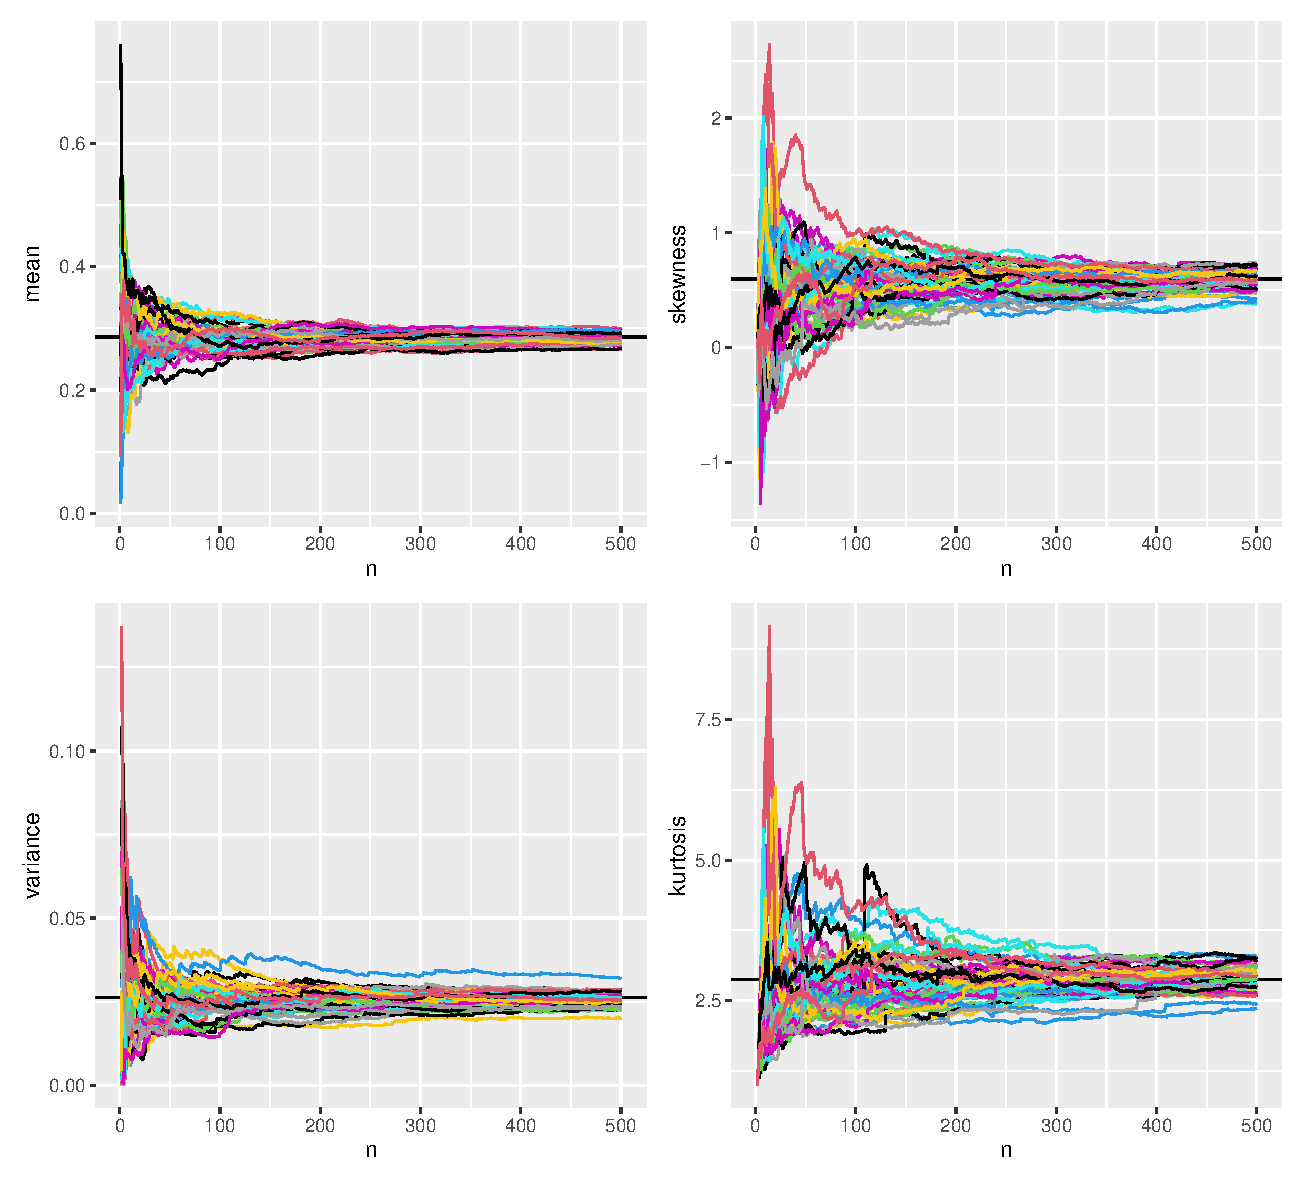
\includegraphics[width=\textwidth]{Rplot.pdf}
  \caption{$\alpha$=2 and $\beta$=5 Convergence Simulation}
  \label{plot1}
  \end{center}
\end{figure}

\end{document}
